\documentclass[11pt,border=5pt]{standalone}
\usepackage{fontspec}
\setmainfont{cmunrm.otf}[BoldFont=cmunbx.otf,ItalicFont=cmunti.otf,BoldItalicFont=cmunbi.otf]
\usepackage{amsmath}
\usepackage{unicode-math}
\setmathfont{NewCMMath-Regular.otf}
\usepackage{tikz}
\usetikzlibrary{arrows.meta,patterns,angles,quotes}
\begin{document}
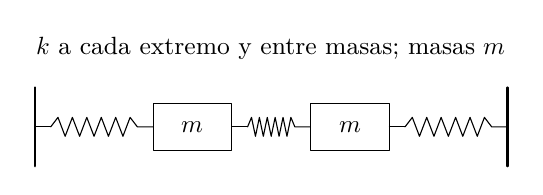
\begin{tikzpicture}[>=Stealth,font=\small,line cap=round,line join=round]
\draw[thick] (-3,-0.5) -- (-3,0.5);
\draw[thick] (3,-0.5) -- (3,0.5);
\draw[] (-3,0) -- (-2.8,0);
\draw (-2.800,0.000) -- (-2.708,0.120) -- (-2.617,-0.120) -- (-2.525,0.120) -- (-2.433,-0.120) -- (-2.342,0.120) -- (-2.250,-0.120) -- (-2.158,0.120) -- (-2.067,-0.120) -- (-1.975,0.120) -- (-1.883,-0.120) -- (-1.792,0.120) -- (-1.700,0.000) -- (-1.500,0.000);
\draw[fill=white] (-1.5,-0.3) rectangle (-0.5,0.3);
\node at (-1,0) {$m$};
\draw[] (-0.5,0) -- (-0.3,0);
\draw (-0.300,0.000) -- (-0.250,0.120) -- (-0.200,-0.120) -- (-0.150,0.120) -- (-0.100,-0.120) -- (-0.050,0.120) -- (0.000,-0.120) -- (0.050,0.120) -- (0.100,-0.120) -- (0.150,0.120) -- (0.200,-0.120) -- (0.250,0.120) -- (0.300,0.000) -- (0.500,0.000);
\draw[fill=white] (0.5,-0.3) rectangle (1.5,0.3);
\node at (1,0) {$m$};
\draw[] (1.5,0) -- (1.7,0);
\draw (1.700,0.000) -- (1.792,0.120) -- (1.883,-0.120) -- (1.975,0.120) -- (2.067,-0.120) -- (2.158,0.120) -- (2.250,-0.120) -- (2.342,0.120) -- (2.433,-0.120) -- (2.525,0.120) -- (2.617,-0.120) -- (2.708,0.120) -- (2.800,0.000) -- (3.000,0.000);
\node at (0,1) {$k$ a cada extremo y entre masas; masas $m$};

\end{tikzpicture}
\end{document}
